
Die Berechnung der aktuellen Orientation des Arduinos war eine grössere Herausforderung,
als wir dies im Vorfeld geplant hatten. Das Problem war hauptsächlich, dass das Gyroskop, welches auf dem SOC verbaut wird, nicht sehr genaue Werte ausgibt.

\subsubsection{Ursprünglicher Lösungsansatz (Gyroskop)}
Ursprünglich haben wir geplant, dass wir anhand der Gyroskop-Daten 
(Das Gyroskop gibt die aktuellen Winkelgeschwindigkeiten für jede Drehachse in Grad/Sekunde aus) 
die aktuellen Winkel wie folgt berechnen können:\\

Die aktuellen Winkel (\begin{math}CurrAngle_{x,y,z}\end{math}) werden zu begin mit 0 initialisiert, In der loop-Funktion des Arduinos werden die aktuellen Winkel mit dem Produkt aus der Winkelgeschwindikeit (\begin{math}v_{x,y,z}\end{math}) und dem Zeitdelta (\begin{math}\Delta{t}\end{math}) addiert.\\

\begin{math}
  CurrAngle_x = CurrAngle_x + v_x \Delta t  \\
  CurrAngle_y = CurrAngle_y + v_y \Delta t  \\
  CurrAngle_z = CurrAngle_z + v_z \Delta t  \\
\end{math}

Diese Methodik hat jedoch dazu geführt, dass die Winkel, durch die Ungenauigkeit der Daten, schon nach kurzer Zeit davon driften.
Um diese Problematik etwas in den Griff zu bekommen, haben wir eine Kalibrierungsfunktion implementiert, welche beim Starten des Arduinos durchloffen wird.
Zum Kalibrieren darf der Arduino nicht bewegt werden. In der Funktion werden nun 500-mal die Gyroskopdaten abgefragt.
Der Durchschnittswert dieser Daten wird anschliessend von zukünftigen Messungen abgezogen.
Mit Hilfe der Kalibrierungsfunktion konnten wir bereits etwas genauere Resultate erzielen, brauchbar waren diese jedoch  noch nicht.

\subsubsection{Erweiterter Lösungsansatz (Beschleunigungssensor)}
Da wir durch das Gyroskop keine genauen Winkel-Werte berechnen konnten, haben wir einen weiteren Lösungsansatz ins Auge gefasst:\\
Durch den Beschleunigungssensor können wir den aktuellen Beschleunigungsvektor auslesen. Solange der Beschleunigungssensor nicht künstlich beschleunigt wird, 
so zeigt dieser Vektor mit Länge (\begin{math}9.81\frac{m}{s^2}\end{math}) immer Richtung Erdmitte. Anhand des Vektors können wir nun die aktuellen Winkelangaben (mit einigen Einschränkungen) sehr genau berechnen.

\vspace{5mm}
\begin{math}
ang_x = arccos{\frac{vect_x}{\lvert\overrightarrow{vect}\rvert}}\\
ang_y = arccos{\frac{vect_y}{\lvert\overrightarrow{vect}\rvert}}
\end{math}
\vspace{5mm}

Die Einschränkungen dieser Methodik liegen auf der Hand, so können die Winkel wie gesagt nur berechnet werden, sofern der Arduino in nicht horizontal oder vertikal beschleunigt wird.
Des Weiteren ist es nicht möglich die Rotation in der Z-Achse (Senkrecht zur Erdmitte) zu berechnen.\\
Um die Rotation in der Z-Achse berechnen zu können, müssten wir einen weiteren Sensor hinzuziehen: den Magnetometer. 
In unserem Projekt haben wir jedoch aufgrund des Zeitmangels darauf verzichtet und uns mit den X und Y werten begnügt.\\
Das Problem der Beschleunigung konnten wir jedoch fast komplett in den Griff bekommen.

\subsubsection{Definitiver Lösungsansatz}
Durch berechnen der Winkel mittels des Beschleunigungssensors konnten wir, solange der Arduino nicht bewegt wird, ziemlich genaue Resultate erzielen.
In unserem definitiven Lösungsansatz haben wir das Problem der Bewegung wie folgt lösen können:\\
Wie bereits gesagt, hat der Vektor der Beschleunigung im Ruhezustand einen Betrag von 1G, ist dieser Betrag höher oder tiefer, so wird der Arduino beschleunigt.
somit berechnen wir die Winkel anhand des Beschleunigungssensors nur, wenn dieser nicht künstlich beschleunigt wird.
Ansonsten nehmen wir die Daten des Gyroskops, um eine Schätzung vorzunehmen.
Damit die Bewegungen geglättet werden, haben wir ausserdem sogenannte PID-Loops verwendet.


\subsubsection{PID-Loop}
PID-Loops, PID-Controller oder auch PID Regler sind häufig in der Regelungstechnik anzutreffen.\\
Sie werden hauptsächlich eingesetzt, um Fehler zu korrigieren und dabei das Überschiessen und das daraus folgende Oszillieren zu verhindern.\\

\begin{figure}[H]
\centering
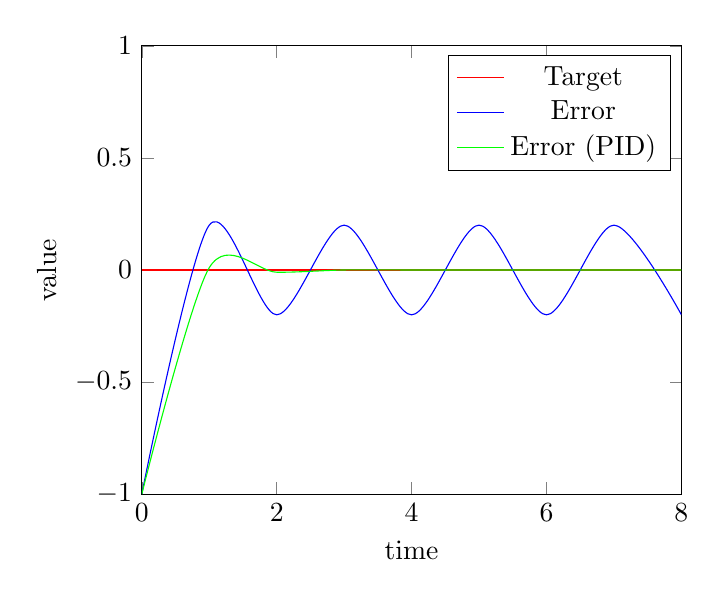
\begin{tikzpicture}
  \begin{axis}[
    xmin = 0,
    xmax = 8,
    ymin = -1,
    ymax = 1,
    xlabel={time},
    ylabel = {value}
    ]
    \addplot[color=red]
  coordinates {(0,0) (8,0) };
  \addlegendentry{Target}
  \addplot[smooth,blue]
  coordinates {(0,-1) (1,0.2) (2,-0.2) (3,0.2) (4,-0.2) (5,0.2) (6,-0.2) (7,0.2) (8,-0.2)};
  \addlegendentry{Error}
  \addplot[smooth,green]
  coordinates {(0,-1) (1,0.01) (2,-0.01) (3,0) (4,0) (5,0) (6,0) (7,0) (8,0)};
  \addlegendentry{Error (PID)}
  
  \end{axis}
  \end{tikzpicture}
  \caption{Regelung mit und ohne PID-Loop}
\end{figure}

In unserem Projekt verwenden wir für alle Drehachsen des Arduinos jeweils ein PID-Loop. 
Die Sensordaten werden nicht direkt in einen Output verwandelt, stattdessen werden sie zum Korriegieren der aktuellen Winkel, welche zwischengespeichert werden, verwendet.
Wie bereits im Lösungsansatz beschrieben, verwenden wir je nachdem ob eine Beschleunigung vorliegt die Gyro- oder Beschleunigungsdaten.\\
Werden die Beschleunigungsdaten verwendet so wird der Fehler, welcher durch den PID-Loop verarbeitet wird folgendermassen berechnet:

\vspace{5mm}
\begin{math} err_{x,y} = accelAngle_{x,y} - currAngle_{x,y} \end{math}
\vspace{5mm}

Werden hingegen die Gyroskopdaten verwendet so kann als Fehler die Winkelgeschwindigkeit im Delta der Zeit verwendet werden.

\vspace{5mm}
\begin{math} err_{x,y} = wV_{x,y}\Delta{t}\end{math}
\vspace{5mm}


\begin{figure}[H]
  \begin{center}
    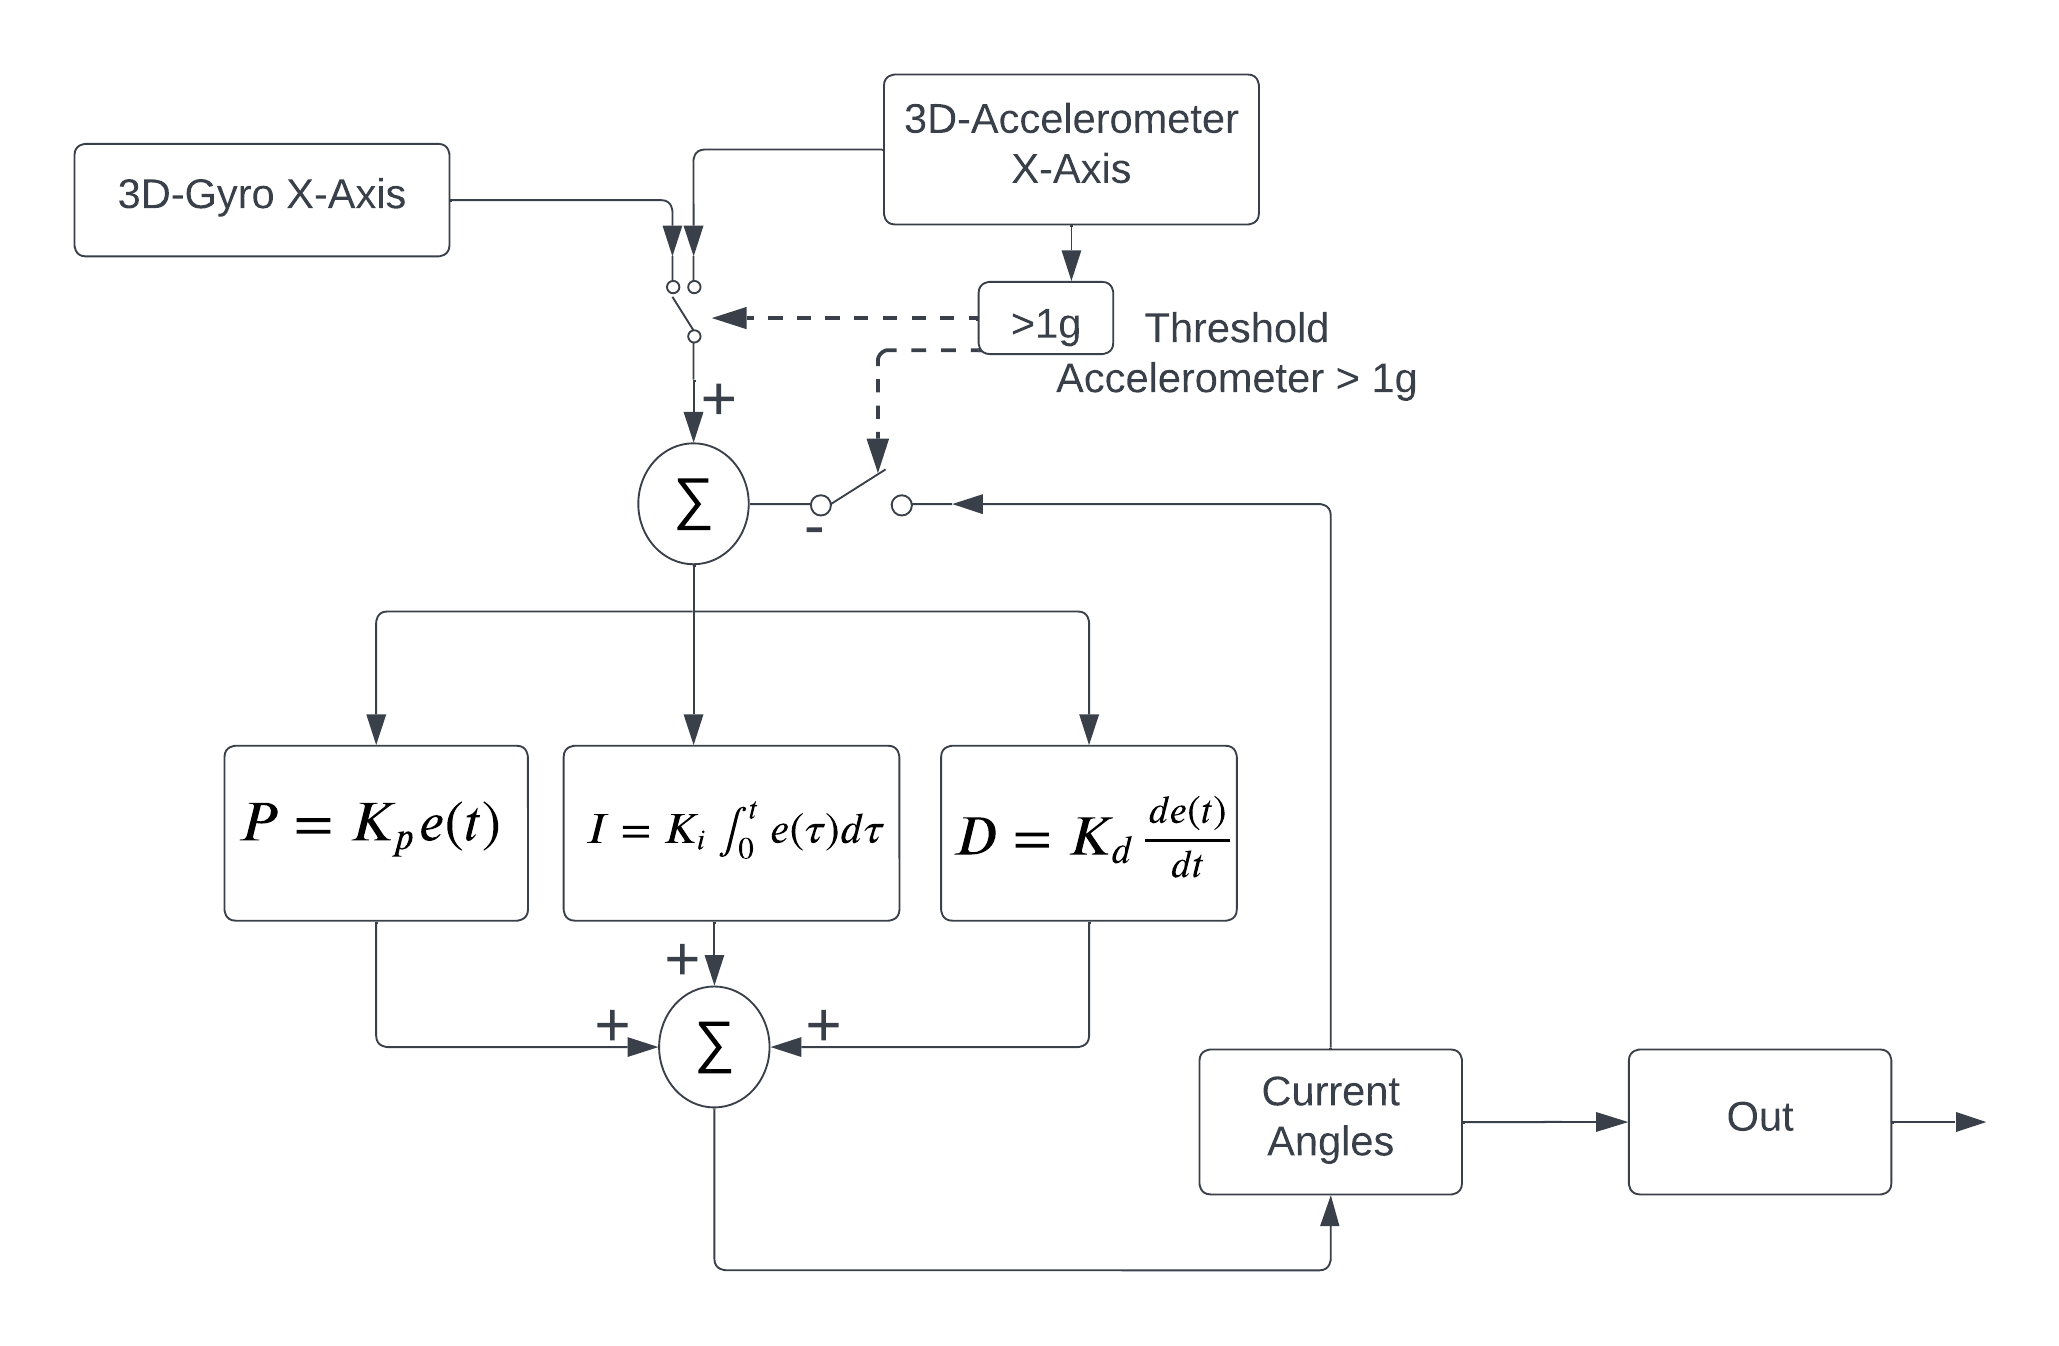
\includegraphics[width=1\linewidth]{content/images/PID_Loop.png}
    \caption{PID Loop}
  \end{center}
\end{figure}

  
\subsubsection{PID-Algorythmus}
\begin{minipage}[l]{0.5\textwidth}
  \begin{math}
    Korrekturwert = K_p e(t) + K_i e_i \Delta{t} + \frac{K_d \Delta{e}}{\Delta{t}} \\
  \end{math} 
\end{minipage}
\begin{minipage}[r]{0.49\textwidth}
  \begin{table}[H]
    \centering
  \settowidth\tymin{Variablen}
  \setlength\extrarowheight{2pt}
  \begin{tabulary}{1.0\textwidth}{|L|L|}
    \hline
    \begin{math} K_p \end{math} & Proportional-Konstante\\
    \hline
    \begin{math} K_i \end{math} & Integral-Konstante\\
    \hline
    \begin{math} K_d \end{math} & Differential-Konstante\\
    \hline
    \begin{math} e(t) \end{math} & aktueller Fehler\\
    \hline
    \begin{math} \Delta{t} \end{math} & Zeit seit der letzten Korrektur\\
    \hline
    \begin{math} \Delta{e} \end{math} & Differenz des aktuellen und letzten Fehlers\\
    \hline
    \begin{math} e_i \end{math} & Fehlerintegral (\begin{math} \int_{0}^t e(t) \end{math})\\
    \hline
  \end{tabulary}
  \caption{Variablen Verzeichnis}
\end{table}
\end{minipage}